%----------------------------------------------------------------------------------------
%	PACKAGES AND OTHER DOCUMENT CONFIGURATIONS
%----------------------------------------------------------------------------------------

\documentclass{article}

\usepackage{fancyhdr} % Required for custom headers
\usepackage{lastpage} % Required to determine the last page for the footer
\usepackage{extramarks} % Required for headers and footers
\usepackage[usenames,dvipsnames]{color} % Required for custom colors
\usepackage{graphicx} % Required to insert images
\usepackage{listings} % Required for insertion of code
\usepackage{courier} % Required for the courier font
\usepackage{lipsum} % Used for inserting dummy 'Lorem ipsum' text into the template
\usepackage{parskip}
% Margins
\topmargin=-0.45in
\evensidemargin=0in
\oddsidemargin=0in
\textwidth=6.5in
\textheight=9.0in
\headsep=0.25in

\linespread{1.1} % Line spacing

% Set up the header and footer
\pagestyle{fancy}
\chead{} % Top left header
\lhead{\hmwkClass\  \hmwkTitle} % Top center head
\rhead{} % Top right header
\lfoot{\lastxmark} % Bottom left footer
\cfoot{} % Bottom center footer
\rfoot{Page\ \thepage\ of\ \protect\pageref{LastPage}} % Bottom right footer
\renewcommand\headrulewidth{0.4pt} % Size of the header rule
\renewcommand\footrulewidth{0.4pt} % Size of the footer rule

\setlength\parindent{0pt} % Removes all indentation from paragraphs

%----------------------------------------------------------------------------------------
%	CODE INCLUSION CONFIGURATION
%----------------------------------------------------------------------------------------

% \definecolor{MyDarkGreen}{rgb}{0.0,0.4,0.0} % This is the color used for comments
\lstloadlanguages{C} % Load C syntax for listings, for a list of other languages supported see: ftp://ftp.tex.ac.uk/tex-archive/macros/latex/contrib/listings/listings.pdf
\lstset{language=C,frame=single,keywordstyle=[1]\color{Blue}\bf} % Use C in this example      



\newcommand{\csnippet}[2]{
\begin{itemize}
\item[]\lstinputlisting[caption=#2,label=#1]{#1.c}
\end{itemize}
}

%----------------------------------------------------------------------------------------
%	DOCUMENT STRUCTURE COMMANDS
%----------------------------------------------------------------------------------------

% Header and footer for when a page split occurs within a problem environment
\newcommand{\enterProblemHeader}[1]{
\nobreak\extramarks{#1}{#1 continued on next page\ldots}\nobreak
\nobreak\extramarks{#1 (continued)}{#1 continued on next page\ldots}\nobreak
}

% Header and footer for when a page split occurs between problem environments
\newcommand{\exitProblemHeader}[1]{
\nobreak\extramarks{#1 (continued)}{#1 continued on next page\ldots}\nobreak
\nobreak\extramarks{#1}{}\nobreak
}

\setcounter{secnumdepth}{0} % Removes default section numbers
\newcounter{homeworkProblemCounter} % Creates a counter to keep track of the number of problems

\newcommand{\homeworkProblemName}{}
\newenvironment{homeworkProblem}[1][Problem \arabic{homeworkProblemCounter}]{ % Makes a new environment called homeworkProblem which takes 1 argument (custom name) but the default is "Problem #"
\stepcounter{homeworkProblemCounter} % Increase counter for number of problems
\renewcommand{\homeworkProblemName}{#1} % Assign \homeworkProblemName the name of the problem
\section{\homeworkProblemName} % Make a section in the document with the custom problem count
\enterProblemHeader{\homeworkProblemName} % Header and footer within the environment
}{
\exitProblemHeader{\homeworkProblemName} % Header and footer after the environment
}

\newcommand{\problemAnswer}[1]{ % Defines the problem answer command with the content as the only argument
\noindent\framebox[\columnwidth][c]{\begin{minipage}{0.98\columnwidth}#1\end{minipage}} % Makes the box around the problem answer and puts the content inside
}

\newcommand{\homeworkSectionName}{}
\newenvironment{homeworkSection}[1]{ % New environment for sections within homework problems, takes 1 argument - the name of the section
\renewcommand{\homeworkSectionName}{#1} % Assign \homeworkSectionName to the name of the section from the environment argument
\subsection{\homeworkSectionName} % Make a subsection with the custom name of the subsection
\enterProblemHeader{\homeworkProblemName\ [\homeworkSectionName]} % Header and footer within the environment
}{
\enterProblemHeader{\homeworkProblemName} % Header and footer after the environment
}

%----------------------------------------------------------------------------------------
%	NAME AND CLASS SECTION
%----------------------------------------------------------------------------------------

\newcommand{\hmwkTitle}{Assignment\ \#4} % assignment title
\newcommand{\hmwkDueDate}{Monday,\ December\ 8,\ 2014} % due date
\newcommand{\hmwkClass}{Programming Concurrent Systems} % class
\newcommand{\hmwkClassTime}{} % lecture time
\newcommand{\hmwkClassInstructor}{} % lecturer
\newcommand{\hmwkAuthorName}{Alyssa - Ilias} %name

%----------------------------------------------------------------------------------------
%	TITLE PAGE
%----------------------------------------------------------------------------------------

\title{
\vspace{2in}
\textmd{\textbf{\hmwkClass:\ \hmwkTitle}}\\
\normalsize\vspace{0.1in}\small{Due\ on\ \hmwkDueDate}\\
\vspace{0.1in}\large{\textit{\hmwkClassInstructor\ \hmwkClassTime}}
\vspace{3in}
}

\author{\textbf{\hmwkAuthorName}}


%----------------------------------------------------------------------------------------

\begin{document}

\maketitle

%----------------------------------------------------------------------------------------
%	TABLE OF CONTENTS
%----------------------------------------------------------------------------------------

%\setcounter{tocdepth}{1} % Uncomment this line if you don't want subsections listed in the ToC

%\newpage
%\tableofcontents
\newpage

%----------------------------------------------------------------------------------------
%	Introduction
%----------------------------------------------------------------------------------------
\begin{homeworkProblem}[Introduction]
	intro

\end{homeworkProblem}
%----------------------------------------------------------------------------------------
%	Heat
%----------------------------------------------------------------------------------------

% To have just one problem per page, simply put a \clearpage after each problem

\begin{homeworkProblem}[Heat dissipation | OpenACC]
\textbf{Solution description}

We also parallelize the reduction step as shown in the snippet below.

\csnippet{reduction}{Reduction using acc directive}

\textbf{Evaluation - Experiments}

We run our experiments on the DAS-4 system using a normal node which has 8 physical cores.

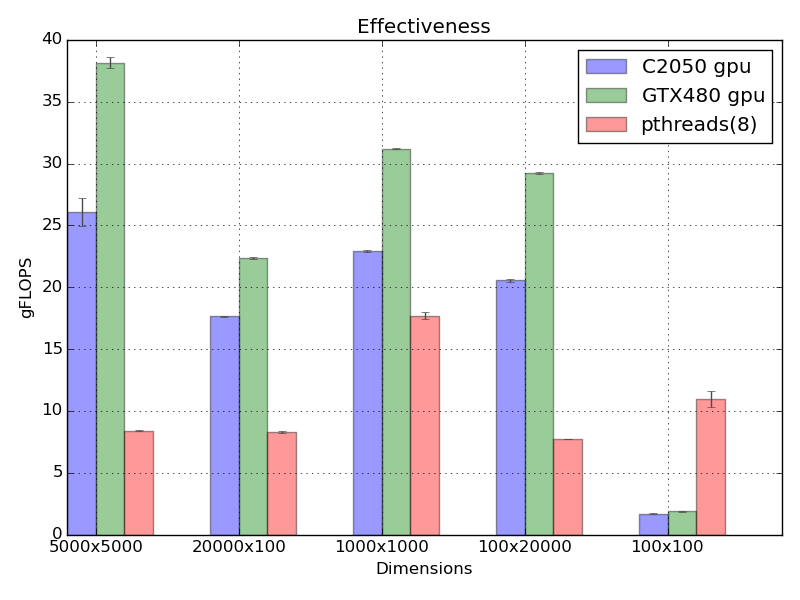
\includegraphics[width=0.75\columnwidth]{effectivness.png}


The figure above shows the effectivness of the parallelism. The experiments where made with the following parameters:

\begin{verbatim}
./heat -e 0.0 -i 2000 -k 2001
\end{verbatim}

Unfortunately we couldn't exeperiment with a lot different accelerators since most of them were being used all the time.

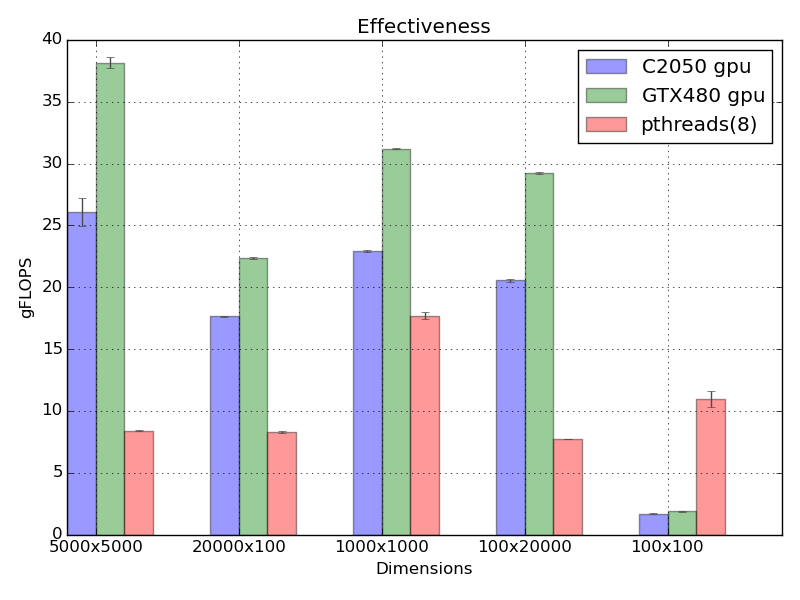
\includegraphics[width=0.75\columnwidth]{effectivness.png}

Notice how for the first time effectiveness does not necessarily mean small execution time because of the communication overhead.


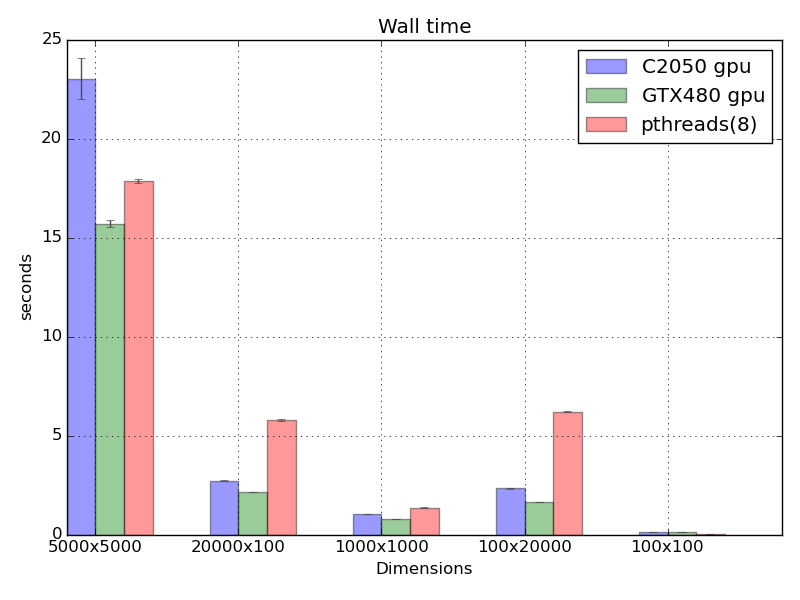
\includegraphics[width=0.75\columnwidth]{walltime.png} 

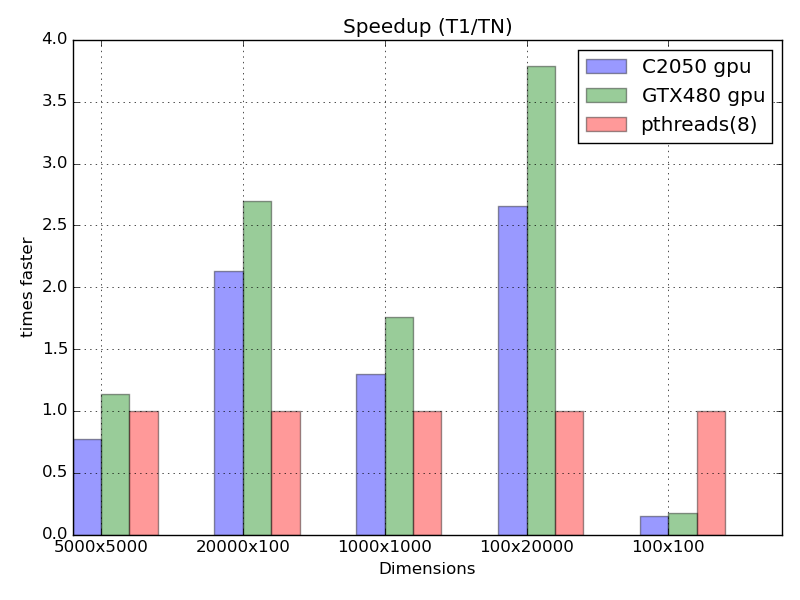
\includegraphics[width=0.75\columnwidth]{speedup_heat.png} 

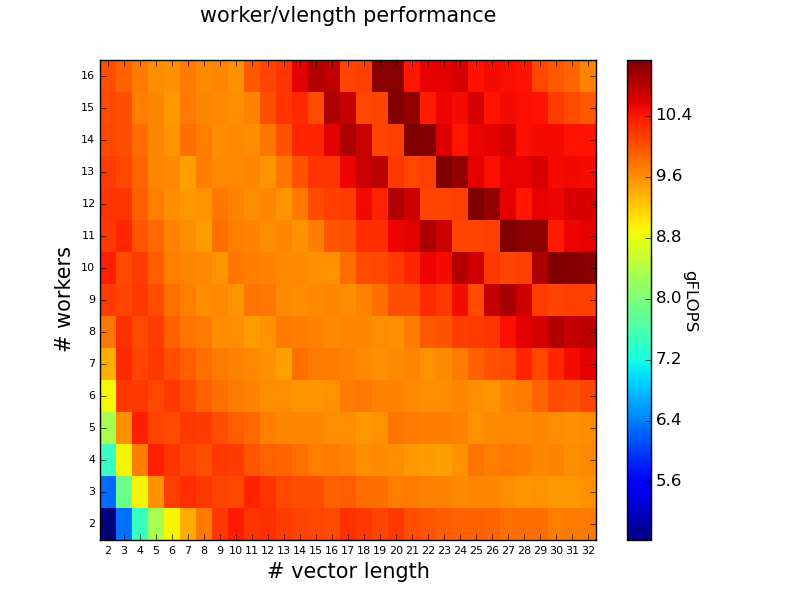
\includegraphics[width=0.75\columnwidth]{heat.png}

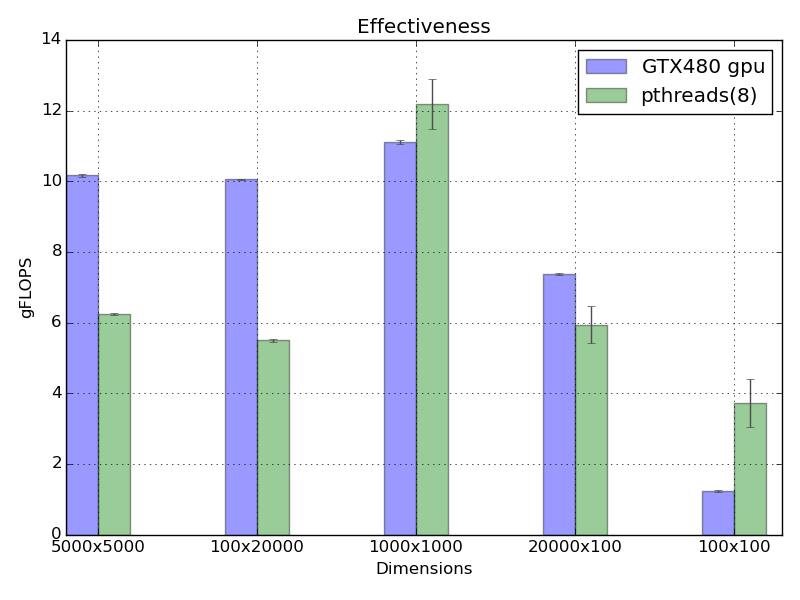
\includegraphics[width=0.75\columnwidth]{effectivness_withreductions.png} 

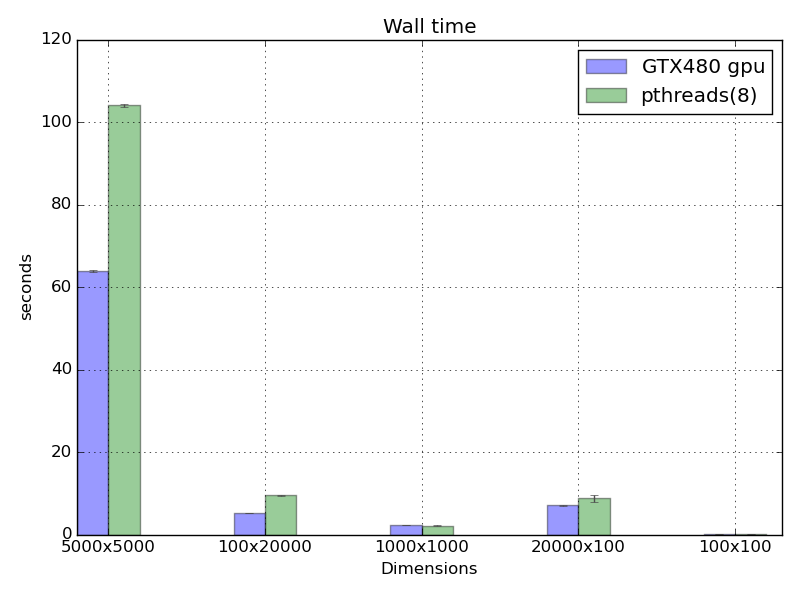
\includegraphics[width=0.75\columnwidth]{walltime_withreductions.png}

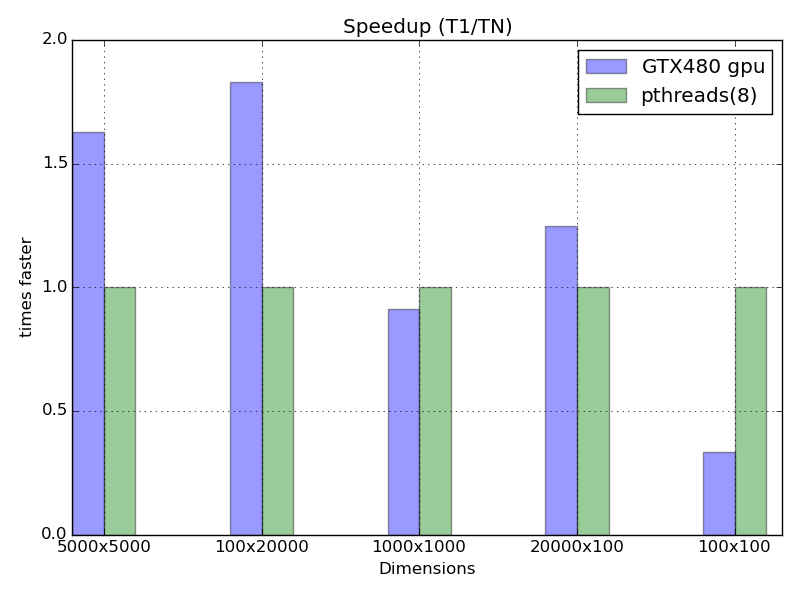
\includegraphics[width=0.75\columnwidth]{speedup_withreductions.png} 



\end{homeworkProblem}

%----------------------------------------------------------------------------------------
%	Merge
%----------------------------------------------------------------------------------------

\begin{homeworkProblem}[Matmul]

Small intro here

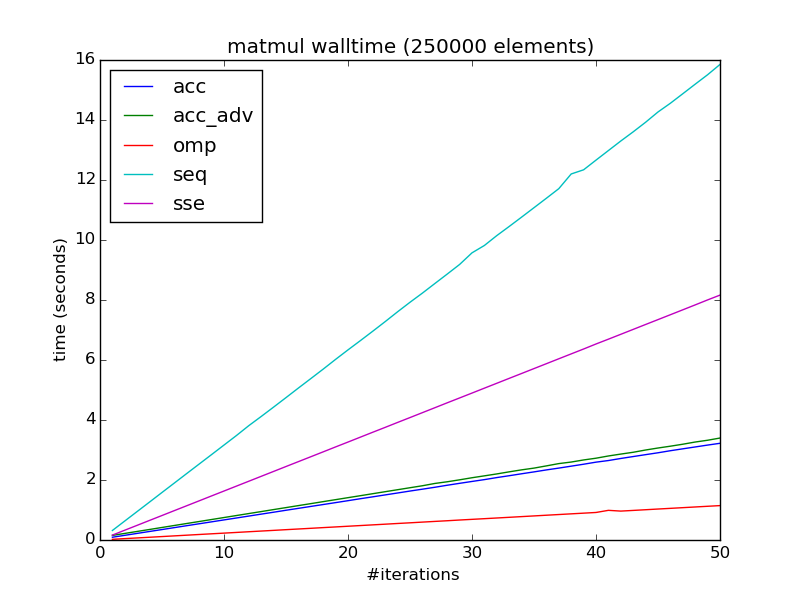
\includegraphics[width=0.75\columnwidth]{fig.png}

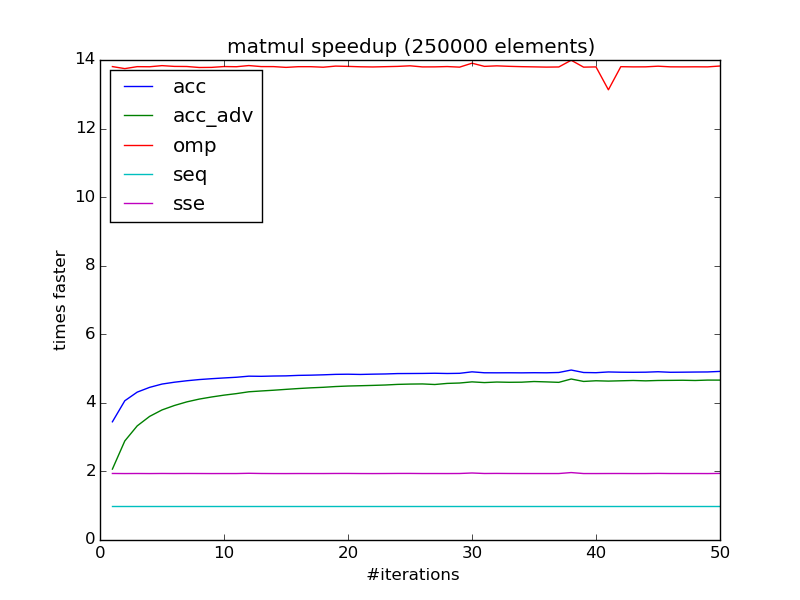
\includegraphics[width=0.75\columnwidth]{speedup.png} 

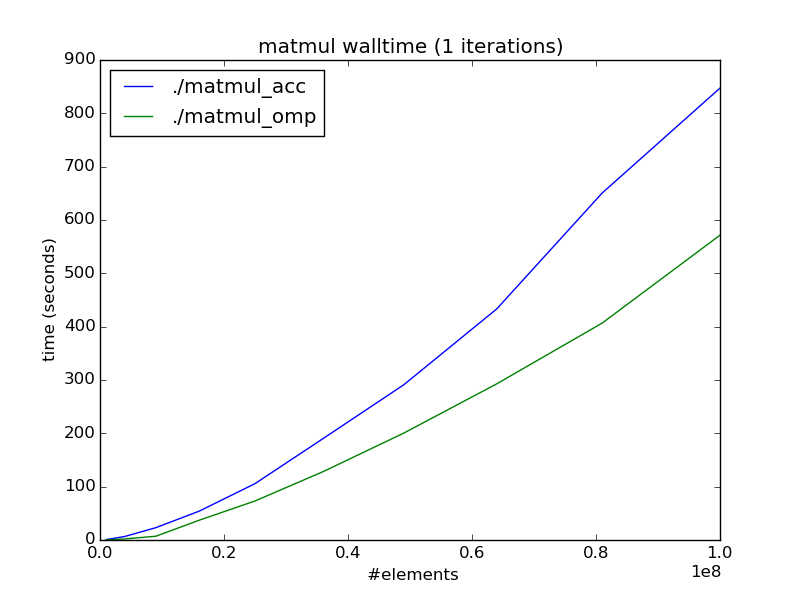
\includegraphics[width=0.75\columnwidth]{bigfig.png} 

%one more fig coming here just like fig1 but with more elements	

\end{homeworkProblem}

%----------------------------------------------------------------------------------------

\end{document}
